\section{Object Constraint Language (OCL)}

\subsection{Overview}

\hspace{1cm} As explained in the previous section, UML is a graphical language for 
visualizing system structure and behavior. However, visual modeling with UML alone 
is insufficient for developing accurate and consistent software models, as UML 
diagrams cannot express all necessary constraints. The Object Management Group (OMG) 
developed the Object Constraint Language (OCL) to address this limitation. 
OCL is a formal assertion language with precise semantics that extends UML by 
allowing developers to specify constraints that cannot be expressed graphically. 
OCL provides two kinds of descriptions: expressions that evaluate to values, and 
constraints that must evaluate to true. The language includes navigation operators 
to traverse model relationships, comprehensive collection operations, and 
quantifiers for building logical statements. OCL constraints typically appear as 
class invariants (conditions that must always be true for all instances) and 
operation pre/postconditions (conditions that must be true before and after 
execution of operations).

\begin{figure}
    \begin{center}
        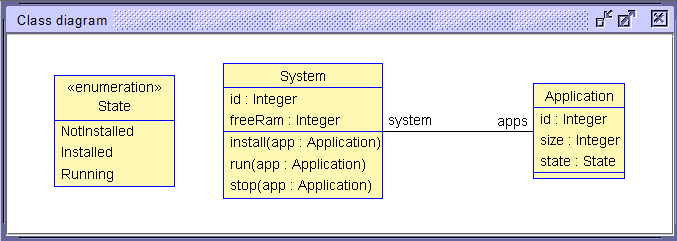
\includegraphics[width=0.8\textwidth]{figures/c1/SoftwareSystem/SS_Ver4.png}
        \caption{Class diagram of the Software System.}
        \label{fig:class_diagram_software_system}
    \end{center}
\end{figure}
We will describe OCL capabilities by means of an example. The UML class diagram in 
Figure \ref{fig:class_diagram_software_system} represents the structure of a simple 
software system. This model contains two classes: \texttt{System} and \texttt{Application}. 
Each class has a \texttt{id} attribute to uniquely identify instances. The \texttt{System}
class has a \texttt{freeRam} attribute corresponding to the amount of free memory that 
is still available, and the following three operations:
\begin{itemize}
    \setlength{\itemsep}{0pt}
    \setlength{\parskip}{0pt}
    \setlength{\parsep}{0pt}
    \item \texttt{install(app : Application)}: installs the application \textit{app} given as parameter.
    \item \texttt{run(app : Application)}: executes the application \textit{app} given as a
    parameter that should be installed.
    \item \texttt{stop(app : Application)}: stops the application \textit{app} given as a
    parameter that should be running.
\end{itemize}

Listing \ref{lst:ocl_software_system} demonstrates three key aspects of OCL constraints. 
First, the memoryConstraint shows a simple value constraint that ensures system 
integrity by preventing negative memory values. Second, the noDuplicateApps 
illustrates OCL's ability to express constraints over collections using built-in 
operations like isUnique(). Third, the sizeConstraint demonstrates how OCL can 
define rules that apply to all instances of a class.
\begin{lstlisting}[
    style=toclstyle, 
    caption={OCL expressions for the Software System}, 
    label={lst:ocl_software_system}
]
context System
inv memoryConstraint: self.freeRam >= 0
inv noDuplicateApps: self.apps->isUnique(app | app.id)   

context Application
inv sizeConstraint: self.size > 0
\end{lstlisting}

These examples represent just a small subset of OCL's expressive capabilities. OCL is type-rich, supporting basic types (Boolean, Real, Integer, String), collection types (Set, Bag, Sequence, OrderedSet), and special types (tuples, OclAny, OclType). The language provides powerful navigation capabilities for traversing relationships in the model, comprehensive collection operations for manipulating groups of objects, and quantifiers (forAll, exists) for building complex logical statements.


%%% Version 3
% The first expression verifies that the \texttt{freeRam} 
% attribute of the \texttt{System} class is greater than or equal to zero, ensuring that the 
% system does not report negative free memory. The second expression checks that the \texttt{apps} 
% collection of the \texttt{System} class contains unique applications by comparing their \texttt{id} 
% attributes. The third expression verifies that the \texttt{size} attribute of the \texttt{Application} 
% class is greater than zero, ensuring that applications have a valid size.

%%% Version 2
% We will describe OCL capabilities by means of an example. The UML class diagram in 
% Figure \ref{fig:class_diagram_software_system} represents the structure of a simple 
% software system. This model contains two classes: \texttt{System} and \texttt{Application}. 
% Each class has a \texttt{id} attribute to uniquely identify instances. The \texttt{System} 
% class has a \texttt{freeMemory} attribute corresponding to the amount of free memory
% that is still available, and the following three operations: 
% \begin{itemize}
%     \setlength{\itemsep}{0pt}
%     \setlength{\parskip}{0pt}
%     \item \texttt{load(app : Application)}: downloads the application \textit{app} given as parameter.
%     \item \texttt{install(app : Application)}: installs a loaded application into the system.
%     \item \texttt{run(app : Application)}: executes the application \textit{app} given as a 
%     parameter that should be both loaded and installed.
% \end{itemize}
% Below are three typical OCL expressions. The first expression verify that 
% % continue this
% \begin{lstlisting}[style=toclstyle]
% context System 
% inv memoryConstraint: self.freeMemory >= 0

% context Application 
% inv sizeConstraint: self.size > 0
% \end{lstlisting}

%%% Version 1
% For example, while a UML class diagram can show that a Bank has multiple Accounts, 
% it cannot express that "an Account must maintain a minimum balance of 
% \$100" - this requires OCL. OCL provides two kinds of descriptions: expressions 
% that evaluate to values, and constraints that must evaluate to true. 
% OCL is type-rich, supporting basic types (Boolean, Real, Integer, String), 
% collection types (Set, Bag, Sequence, OrderedSet), and special types (tuples, 
% OclAny, OclType). The language includes navigation operators to traverse model 
% relationships, comprehensive collection operations, and quantifiers for building 
% logical statements. OCL constraints typically appear as class invariants 
% (conditions that must always be true for all instances) and operation 
% pre/postconditions (conditions that must be true before and after operation execution).

%%% Sample 1
% As explained in Sect. 2.1, UML is a graphical language for visualization of the system
% state. But visual modeling with the UML alone is not enough for the development of
% accurate and consistent software model. For this reason, Object Management Group
% (OMG), in 1997, developed Object Constraint Language (OCL), which describes 
% expressions on UML models and thus extends further the functionality of UML [60].
% [For example, ... (write about limitation of UML and how OCL can help to overcome 
% it in the context of an example)]
% OCL provides two kinds of descriptions, (a) OCL expression, which is defined
%  in the context of the constrained elements and evaluates some values, and (b) OCL
%  constraint, which is restrictive statements concerning some underlying model that
%  should evaluate to true. Basically, an OCL constraint is referred to as an OCL
%  expression of the Boolean type.
% The OCLprovides variables and operations which can be combined in various ways
% to build expressions. There are many OCL expression types. The simplest types are
% the basic type which consists of the types Boolean, Real, Integer and String. The
% concrete collection types are Bag, Sequence, Set and OrderedSet. The other types
% include tuples, which can contain one to many values of other types and special types
% such as OclAny, OclType, OclExpression, and OclState.
% There are three different types of OCL constraints, namely invariants of classes,
%  preconditions and postconditions of operations, which are used to describe model
%  properties. An invariant is a restriction in the form of expression which is applied
%  to all instances of the class diagram and that must be true for all instances, i.e., an
%  invariant must be satisfied after the creation of an instance of the class for which
%  the invariant is defined.

%%% Sample 2
% OCL is a formal assertion language, easy to use, with precise and unambiguous semantics [5]. It allows the annotation
%  of any object-oriented model, even if it is most used within UML diagrams. OCL is very rich, it includes fairly complete
%  support for:
%  – Navigation operators to navigate within the object-oriented model;
%  – Set/sequence operations to manipulate sets and sequences of objects;
%  – Universal/existential quantifiers to build first order (logic) statemeents;

\subsection{OCL Limitations}

%%% Sample
% OCL is a first-order predicate logic.
% As previously mentioned, the OCL expressions are evaluated over a single system state or a one-step transition at some
% point in time. But, the OCL language also provides some implicit quantification over time by means of OCL rules. An OCL
% rule is a temporal quantification applied to an OCL boolean expression, and may be an invariant of a class, a pre- or a
% post-condition of an operation. The expression within an invariant rule has to be satisfied throughout the whole life-time of all instances of the context
% class. A precondition has to be true each time the corresponding operation is called, and a postcondition has to be true
% each time right after the corresponding operation execution has terminated. The operation parameters can be used within a pre or a post-condition rule, but the @pre OCL feature is only used
% within a post-condition rule. When @pre is used within the boolean expression of a post-condition rule, this latter is
% evaluated over two system states, one right before the operation call and one right after its execution. In other words, OCL
% expressions describe a single system state or a one-step transition from a previous state to a new state upon the call of
% some operation. Therefore, there is no way to make OCL expressions involving different states of the model at arbitrary
% points in time. OCL has a very limited temporal dimension.
